\documentclass[11pt]{article}

\usepackage[margin=1in]{geometry}
\usepackage[T1]{fontenc}
\usepackage[utf8]{inputenc}
\usepackage{lmodern}
\usepackage{microtype}
\usepackage{hyperref}
\usepackage{xcolor}
\usepackage{enumitem}
\usepackage{booktabs}
\usepackage{longtable}
\usepackage{array}
\usepackage{listings}
\usepackage{float}
\usepackage{tikz}
\usetikzlibrary{arrows.meta,positioning,fit,shapes.geometric}

\hypersetup{
  colorlinks=true,
  linkcolor=blue!50!black,
  urlcolor=blue!50!black
}

\definecolor{codebg}{RGB}{247,248,250}
\definecolor{boxblue}{RGB}{224,236,255}
\definecolor{boxgreen}{RGB}{226,245,232}
\definecolor{boxorange}{RGB}{255,241,224}
\definecolor{boxgray}{RGB}{242,242,242}

\lstdefinestyle{repo}{
  backgroundcolor=\color{codebg},
  basicstyle=\ttfamily\small,
  frame=single,
  framesep=6pt,
  rulecolor=\color{black!15},
  columns=fullflexible,
  keepspaces=true,
  showstringspaces=false,
  breaklines=true
}

\newcommand{\file}[1]{\texttt{#1}}
\newcommand{\code}[1]{\texttt{#1}}

\title{\textbf{Live Map Flow Guide}\\[4pt]
How the Live VPR Map Is Built, Stored, and Queried}
\author{Project Documentation}
\date{\today}

\begin{document}
\maketitle

\section*{Purpose}
This document explains the \textbf{map flow} used by the live VPR demo. It answers four practical questions:

\begin{itemize}[leftmargin=*]
  \item How is a live reference map created?
  \item What exactly is saved to disk?
  \item How are descriptors extracted and stored?
  \item How are live query frames matched back to the map?
\end{itemize}

It is written as an onboarding document for a new developer. The goal is to make the control flow easy to follow without copying entire source files into the document.

\section{The Short Answer}
The live system stores the map in a \file{.npz} file containing:

\begin{itemize}[leftmargin=*]
  \item a matrix of normalized reference descriptors,
  \item a list of filesystem paths to the saved reference images,
  \item and metadata describing how the map was built.
\end{itemize}

For a \textbf{live-built map}, the system also keeps two external artifacts on disk:

\begin{itemize}[leftmargin=*]
  \item the recorded traversal video, and
  \item the sampled reference image files extracted from that video.
\end{itemize}

So the map is \textbf{not} just images, and it is \textbf{not} just features either. It is a combination of:

\begin{itemize}[leftmargin=*]
  \item \textbf{descriptors in the map file} for fast matching,
  \item \textbf{image files on disk} for visualization and debugging,
  \item \textbf{metadata} to make the map reusable and self-describing.
\end{itemize}

\section{End-to-End Architecture}

\subsection{Overview}
\begin{figure}[H]
\centering
\resizebox{0.98\textwidth}{!}{%
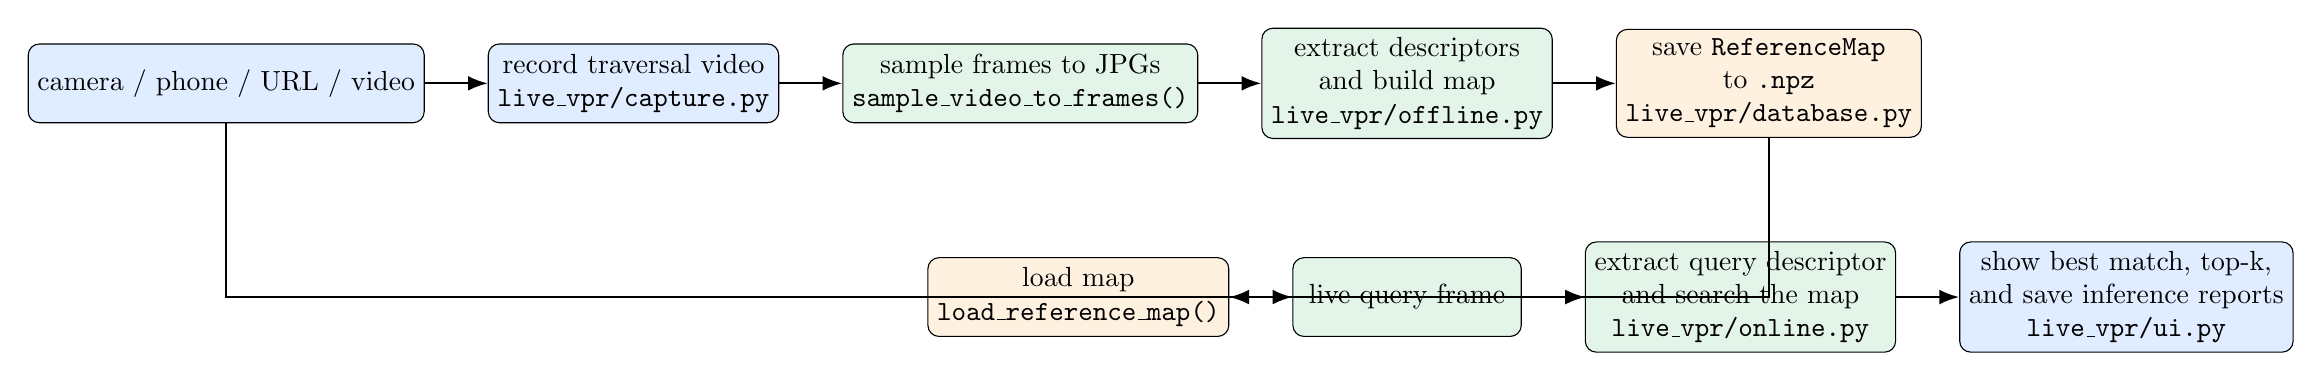
\begin{tikzpicture}[
  node distance=8mm and 8mm,
  box/.style={draw, rounded corners, align=center, minimum width=29mm, minimum height=10mm, fill=boxgray},
  arrow/.style={-{Latex[length=2.5mm]}, thick}
]
\node[box, fill=boxblue] (source) {camera / phone / URL / video};
\node[box, right=of source, fill=boxblue] (record) {record traversal video\\\file{live\_vpr/capture.py}};
\node[box, right=of record, fill=boxgreen] (sample) {sample frames to JPGs\\\code{sample\_video\_to\_frames()}};
\node[box, right=of sample, fill=boxgreen] (build) {extract descriptors\\and build map\\\file{live\_vpr/offline.py}};
\node[box, right=of build, fill=boxorange] (store) {save \file{ReferenceMap}\\to \file{.npz}\\\file{live\_vpr/database.py}};

\node[box, below=15mm of build, fill=boxgreen] (query) {live query frame};
\node[box, left=of query, fill=boxorange] (load) {load map\\\code{load\_reference\_map()}};
\node[box, right=of query, fill=boxgreen] (match) {extract query descriptor\\and search the map\\\file{live\_vpr/online.py}};
\node[box, right=of match, fill=boxblue] (ui) {show best match, top-k,\\and save inference reports\\\file{live\_vpr/ui.py}};

\draw[arrow] (source) -- (record);
\draw[arrow] (record) -- (sample);
\draw[arrow] (sample) -- (build);
\draw[arrow] (build) -- (store);
\draw[arrow] (store) |- (load);
\draw[arrow] (source) |- (query);
\draw[arrow] (query) -- (match);
\draw[arrow] (load) -- (match);
\draw[arrow] (match) -- (ui);
\end{tikzpicture}
}
\caption{The live map flow: capture once, build once, then localize many query frames against the saved map.}
\end{figure}

\subsection{Artifact-Level View}
\begin{figure}[H]
\centering
\resizebox{0.98\textwidth}{!}{%
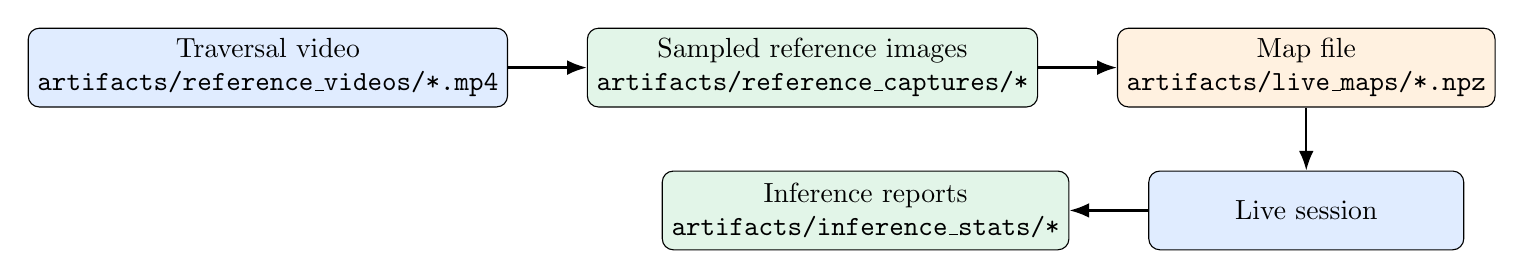
\begin{tikzpicture}[
  node distance=8mm and 10mm,
  box/.style={draw, rounded corners, align=center, minimum width=40mm, minimum height=10mm, fill=boxgray},
  arrow/.style={-{Latex[length=2.5mm]}, thick}
]
\node[box, fill=boxblue] (video) {Traversal video\\\file{artifacts/reference\_videos/*.mp4}};
\node[box, right=of video, fill=boxgreen] (frames) {Sampled reference images\\\file{artifacts/reference\_captures/*}};
\node[box, right=of frames, fill=boxorange] (map) {Map file\\\file{artifacts/live\_maps/*.npz}};
\node[box, below=of map, fill=boxblue] (runtime) {Live session};
\node[box, left=of runtime, fill=boxgreen] (reports) {Inference reports\\\file{artifacts/inference\_stats/*}};

\draw[arrow] (video) -- (frames);
\draw[arrow] (frames) -- (map);
\draw[arrow] (map) -- (runtime);
\draw[arrow] (runtime) -- (reports);
\end{tikzpicture}
}
\caption{Persistent artifacts used by the live map system.}
\end{figure}

\section{Which Files To Read}
If you want to understand the flow in code, read these files in this order:

\begin{enumerate}[leftmargin=*]
  \item \file{live\_vpr\_test.py}
  \item \file{live\_vpr/capture.py}
  \item \file{live\_vpr/offline.py}
  \item \file{live\_vpr/database.py}
  \item \file{live\_vpr/extractors.py}
  \item \file{live\_vpr/online.py}
  \item \file{live\_vpr/search.py}
  \item \file{live\_vpr/ui.py}
\end{enumerate}

\section{Step 1: The CLI Starts the Live Map Build}
The live map flow begins in \file{live\_vpr\_test.py}, inside \code{build\_live\_map()}.

\begin{lstlisting}[style=repo,language=Python,caption={Core structure of \code{build\_live\_map()} in \file{live\_vpr\_test.py}.}]
sampling_result = sample_video_to_frames(
    FrameSamplingConfig(
        video_path=recording_video_path,
        output_dir=args.capture_dir,
        sample_fps=args.sample_fps,
        frame_prefix=args.capture_prefix,
        max_frames=args.max_captures,
        save_scale=args.capture_save_scale,
    )
)

builder = MapBuilder(args.descriptor)
reference_map, stats = builder.build_from_paths(
    image_paths=image_paths,
    output_path=args.map_path,
    image_dir=sampling_result.output_dir,
    target_size=(args.resize_width, args.resize_height),
    metadata_extra={...},
)
\end{lstlisting}

\textbf{What this means:}

\begin{itemize}[leftmargin=*]
  \item The CLI either records a traversal video or reuses an existing video.
  \item It samples that video into a folder of still reference images.
  \item It then passes those saved image paths into \code{MapBuilder}.
  \item \code{MapBuilder} extracts descriptors and writes the final \file{.npz} map.
\end{itemize}

This function is the best place to start because it shows the full orchestration in one place.

\section{Step 2: Traversal Video Recording}
If the user is building the map from a live source, the video is recorded by \code{LiveReferenceRecorder} in \file{live\_vpr/capture.py}.

\begin{lstlisting}[style=repo,language=Python,caption={Traversal recording loop in \file{live\_vpr/capture.py}.}]
while True:
    ok, frame = self.source.read()
    if not ok or frame is None:
        break

    if writer is None:
        writer = cv2.VideoWriter(...)

    if recording:
        writer.write(frame)
        frame_count += 1
\end{lstlisting}

\textbf{Important detail:} the raw traversal frames are first stored as a normal \file{.mp4} video. This is useful because:

\begin{itemize}[leftmargin=*]
  \item the traversal can be reused later,
  \item different sampling rates can be tested without walking the route again,
  \item and the video acts as a reproducible record of how the map was created.
\end{itemize}

\section{Step 3: Sampling the Video Into Reference Images}
After recording, the video is converted into a set of sampled reference images by \code{sample\_video\_to\_frames()} in \file{live\_vpr/capture.py}.

\begin{lstlisting}[style=repo,language=Python,caption={Frame sampling and saved-image downsampling.}]
if should_sample:
    filename = f"{config.frame_prefix}_{len(saved_paths):04d}_{timestamp_ms:08d}ms.jpg"
    output_path = output_dir / filename
    frame_to_save = frame
    if config.save_scale < 1.0:
        frame_to_save = cv2.resize(frame, (new_width, new_height),
                                   interpolation=cv2.INTER_AREA)
    cv2.imwrite(str(output_path), frame_to_save)
    saved_paths.append(str(output_path))
\end{lstlisting}

\textbf{What is happening here:}

\begin{itemize}[leftmargin=*]
  \item The video is sampled by time, not by hardcoded frame index.
  \item Each sampled frame is saved as a real image file in \file{args.capture\_dir}.
  \item The file name includes a frame counter and timestamp.
  \item The new \code{save\_scale} option lets the project store smaller sampled images to reduce disk and memory pressure.
\end{itemize}

\textbf{Practical note.} These sampled images are not just temporary scratch files. The rest of the system keeps their paths and later uses them in the live UI for match thumbnails and exported reports.

\section{Step 4: Loading Images and Extracting Descriptors}
The actual descriptor-building logic lives in \file{live\_vpr/offline.py}, inside \code{MapBuilder.build\_from\_paths()}.

\begin{lstlisting}[style=repo,language=Python,caption={Map building in \file{live\_vpr/offline.py}.}]
images = [_load_rgb_image(path, target_size) for path in image_paths]

descriptors = compute_global_descriptors(self.extractor, images)
descriptors = normalize_descriptors(descriptors)

reference_map = ReferenceMap(
    descriptors=descriptors,
    image_paths=[str(path.resolve()) for path in image_paths],
    metadata=metadata,
)
saved_path = save_reference_map(reference_map, output_path)
\end{lstlisting}

\textbf{This step does four things:}

\begin{enumerate}[leftmargin=*]
  \item Load each sampled image from disk.
  \item Convert it to RGB and resize it to the map target size.
  \item Extract one global descriptor per image.
  \item Normalize the descriptor matrix so cosine-style similarity becomes a dot product.
\end{enumerate}

The image-loading helper is intentionally simple:

\begin{lstlisting}[style=repo,language=Python,caption={Image preprocessing before descriptor extraction.}]
with Image.open(image_path) as image:
    image = image.convert("RGB")
    image = image.resize(target_size, Image.Resampling.BILINEAR)
    return np.array(image)
\end{lstlisting}

This means the map descriptors are built from consistently resized RGB images, even if the saved sampled JPGs were originally larger or smaller.

\section{Step 5: How the Feature Extractor Is Chosen}
The project uses \file{live\_vpr/extractors.py} as the adapter layer between the live pipeline and the actual feature extraction implementations under \file{feature\_extraction/}.

\begin{lstlisting}[style=repo,language=Python,caption={Extractor factory in \file{live\_vpr/extractors.py}.}]
def create_feature_extractor(descriptor_name: str) -> Any:
    if descriptor_name == "CosPlace":
        return CosPlaceFeatureExtractor()
    if descriptor_name == "EigenPlaces":
        return EigenPlacesFeatureExtractor()
    ...
\end{lstlisting}

\begin{lstlisting}[style=repo,language=Python,caption={Descriptor computation wrapper.}]
def compute_global_descriptors(extractor: Any, images: list[np.ndarray]) -> np.ndarray:
    descriptors = extractor.compute_features(images)
    if isinstance(descriptors, tuple):
        descriptors = descriptors[0]
    descriptors = np.asarray(descriptors, dtype=np.float32)
    if descriptors.ndim != 2:
        raise ValueError(...)
    return descriptors
\end{lstlisting}

\textbf{Why this wrapper exists:}

\begin{itemize}[leftmargin=*]
  \item different models expose slightly different outputs,
  \item the live pipeline wants a consistent 2D matrix shape,
  \item and the rest of the code should not need to know model-specific quirks.
\end{itemize}

\section{Step 6: What a Saved Map Actually Contains}
The in-memory map object is defined in \file{live\_vpr/database.py}.

\begin{lstlisting}[style=repo,language=Python,caption={ReferenceMap schema.}]
@dataclass
class ReferenceMap:
    descriptors: np.ndarray
    image_paths: list[str]
    metadata: dict[str, Any]
\end{lstlisting}

The save function writes it as a compressed \file{.npz}:

\begin{lstlisting}[style=repo,language=Python,caption={Serialization in \file{live\_vpr/database.py}.}]
np.savez_compressed(
    output,
    descriptors=reference_map.descriptors.astype(np.float32),
    image_paths=np.array(reference_map.image_paths),
    metadata=json.dumps(reference_map.metadata),
)
\end{lstlisting}

\subsection{What Is Stored}
\begin{longtable}{p{0.26\linewidth} p{0.64\linewidth}}
\toprule
\textbf{Stored item} & \textbf{Meaning} \\
\midrule
\code{descriptors} & One normalized feature vector per reference image. This is the main data used for matching. \\
\code{image\_paths} & Absolute paths to the sampled or original reference images on disk. These are used by the UI and report-export code. \\
\code{metadata} & Descriptor name, resize target, source directory, creation time, and extra live-build facts such as sampling FPS and traversal video path. \\
\bottomrule
\end{longtable}

\subsection{What Is Not Stored Inside the Map File}
\begin{itemize}[leftmargin=*]
  \item The reference image pixels themselves are \textbf{not} embedded inside the \file{.npz}.
  \item The traversal video is \textbf{not} embedded inside the \file{.npz}.
\end{itemize}

That design keeps the map file smaller while still preserving enough information for matching and UI rendering.

\section{Step 7: Metadata Added by Live Map Building}
Live-built maps add extra metadata on top of the standard map fields. The extra values are attached in \file{live\_vpr\_test.py} when calling \code{MapBuilder.build\_from\_paths()}.

\begin{lstlisting}[style=repo,language=Python,caption={Live-build metadata extras.}]
metadata_extra={
    "live_build_video_path": recording_video_path,
    "live_build_sample_fps": sampling_result.sample_fps,
    "live_build_source_fps": sampling_result.source_fps,
    "live_build_video_duration_s": sampling_result.video_duration_s,
    "live_build_saved_frame_scale": args.capture_save_scale,
}
\end{lstlisting}

This is useful for reproducibility: a developer can inspect a map later and understand \textbf{how} it was created.

\section{Step 8: Loading the Map During Live Inference}
When the demo enters online mode, \file{live\_vpr\_test.py} loads the saved map first:

\begin{lstlisting}[style=repo,language=Python,caption={Map loading at runtime.}]
reference_map = load_reference_map(args.map_path)
target_size = tuple(reference_map.metadata.get("target_size", [640, 480]))
search_config = SearchConfig.from_namespace(args)

localizer = LiveLocalizer(
    reference_map=reference_map,
    descriptor_name=descriptor,
    threshold=args.threshold,
    top_k=args.top_k,
    search_config=search_config,
)
\end{lstlisting}

Two important ideas appear here:

\begin{itemize}[leftmargin=*]
  \item The live query frame is resized to the same target size used during map building.
  \item The descriptor type used at runtime is resolved from the map, so the system can localize with the same representation the map was built with.
  \item The map lookup strategy is not hardcoded; it is configured through \code{SearchConfig}.
\end{itemize}

\section{Step 9: How Matching Works Online}
The matching logic lives in \file{live\_vpr/online.py}, inside \code{LiveLocalizer.localize\_rgb()}.

\begin{lstlisting}[style=repo,language=Python,caption={Online matching in \file{live\_vpr/online.py}.}]
descriptor = compute_global_descriptors(self.extractor, [rgb_image])
descriptor = descriptor / (np.linalg.norm(descriptor, axis=1, keepdims=True) + 1e-8)
search_result = self.search_backend.search(descriptor[0], top_k=self.top_k)
\end{lstlisting}

\textbf{What this does:}

\begin{enumerate}[leftmargin=*]
  \item Extract one descriptor for the current query frame.
  \item Normalize it.
  \item Hand the query descriptor to the configured search backend.
  \item Receive the best match and top-k candidates back from that backend.
\end{enumerate}

Because both map descriptors and query descriptors are normalized, every backend is still trying to solve the same geometric problem: find the reference descriptors with the largest cosine-style similarity to the query. The difference is \emph{how} the candidate set is found.

\subsection{The Search Layer}
The backend abstraction lives in \file{live\_vpr/search.py}. The localizer constructs it once and then reuses it for every frame:

\begin{lstlisting}[style=repo,language=Python,caption={Search backend construction.}]
self.search_config = search_config or SearchConfig()
self.search_backend = create_search_backend(reference_map.descriptors, self.search_config)
\end{lstlisting}

\textbf{Current backends:}

\begin{longtable}{p{0.18\linewidth} p{0.28\linewidth} p{0.42\linewidth}}
\toprule
\textbf{Backend} & \textbf{What it does} & \textbf{Where it shines} \\
\midrule
\texttt{exact} & Scores the query against the full descriptor matrix with a partial top-k selection. & Small or medium maps where simplicity and exactness matter more than raw speed. \\
\texttt{hnsw} & Uses a graph-based approximate nearest-neighbor index. & Larger maps where low query latency matters and a practical CPU ANN backend is needed. \\
\texttt{faiss\_ivf\_flat} & Searches only the most relevant FAISS clusters while still storing full vectors inside them. & Large static maps where you want a strong speed/accuracy tradeoff. \\
\texttt{faiss\_ivf\_pq} & Searches clustered descriptors that are also compressed with product quantization. & Very large maps where memory use matters in addition to search speed. \\
\bottomrule
\end{longtable}

\subsection{What Reranking Means}
Approximate retrieval often works best as a two-stage pipeline:

\begin{enumerate}[leftmargin=*]
  \item a \textbf{fast candidate stage} that narrows the search to a shortlist,
  \item then a \textbf{precise reranking stage} that computes exact scores only on that shortlist.
\end{enumerate}

That second step is called \textbf{reranking}. In this project it is implemented by \code{\_rerank\_exact(...)}:

\begin{lstlisting}[style=repo,language=Python,caption={Exact reranking in \file{live\_vpr/search.py}.}]
if self.config.rerank:
    indices, scores = _rerank_exact(self.descriptors, query, candidate_indices, top_k)
\end{lstlisting}

\textbf{Why reranking helps:}

\begin{itemize}[leftmargin=*]
  \item ANN backends are fast because they do \emph{not} score every map descriptor.
  \item But the approximate ordering of candidates is not always the same as the true cosine ordering.
  \item Exact reranking restores the final ordering using the original descriptor matrix.
  \item It also gives more trustworthy final scores for thresholding and UI display.
\end{itemize}

\textbf{Why reranking cannot do everything:} if the fast stage never retrieves the true match, reranking cannot recover it. Reranking improves the \emph{ordering of retrieved candidates}, not the \emph{coverage of candidates that were never retrieved}. That is why \code{search\_candidate\_k} is still important.

\subsection{A Tiny Worked Example}
Suppose the map has eight reference descriptors \(\{A,B,C,D,E,F,G,H\}\), and the live query really belongs near \(E\).

\paragraph{Exact search.}
The system computes all eight scores and sorts them:

\[
E:0.92,\; F:0.86,\; D:0.71,\; B:0.52,\; C:0.49,\; G:0.31,\; A:0.18,\; H:0.10
\]

This is exact, simple, and easy to reason about, but it always touches the full map.

\paragraph{HNSW.}
The graph index might quickly retrieve candidates \(\{F,E,D\}\). Those are already very good, so reranking them exactly produces:

\[
E:0.92,\; F:0.86,\; D:0.71
\]

This is much cheaper than scanning all eight references if the real map has tens of thousands of entries instead of eight.

\paragraph{FAISS IVF Flat.}
Suppose the reference descriptors are partitioned into clusters and the query only probes the cluster containing \(\{D,E,F,G\}\). Search is now restricted to that smaller region, but the vectors inside that region are still stored exactly. This is a strong option when the map is large and fairly static.

\paragraph{FAISS IVF PQ.}
Suppose the same relevant cluster is probed, but the descriptors inside it are stored in compressed form. This lowers memory usage, which matters when maps get very large, but it can make the approximate shortlist a bit noisier. Reranking is especially useful here because it restores the final ordering with exact scores.

\subsection{When To Choose Each Backend}
\begin{itemize}[leftmargin=*]
  \item Start with \texttt{exact} if the map is still small enough and you want the easiest baseline.
  \item Move to \texttt{hnsw} first when latency becomes the problem and you want a practical ANN backend on CPU.
  \item Use \texttt{faiss\_ivf\_flat} when the map is larger and you want a more scalable clustering-based search.
  \item Use \texttt{faiss\_ivf\_pq} when both speed and memory become real constraints.
\end{itemize}

\subsection{Decision Rule}
The localizer also produces a simple threshold-based recognition decision:

\begin{lstlisting}[style=repo,language=Python,caption={Recognition decision.}]
recognized = float(search_result.scores[0]) >= self.threshold
\end{lstlisting}

This means the runtime system does \textbf{retrieval + thresholding}, not offline benchmark evaluation. It returns:

\begin{itemize}[leftmargin=*]
  \item the best reference index,
  \item the best similarity score,
  \item whether that score passes the threshold,
  \item and the top-k ranked candidates.
\end{itemize}

\section{Step 10: Why the Reference Image Paths Matter}
The live UI uses the stored \code{image\_paths} to reload the reference images later. This happens in \file{live\_vpr/ui.py}.

\begin{lstlisting}[style=repo,language=Python,caption={Reference image loading in the UI.}]
def _load_reference_image(self, index: int) -> np.ndarray | None:
    ref_path = self.reference_map.image_paths[index]
    return cv2.imread(ref_path)
\end{lstlisting}

Those loaded reference images are then shown in:

\begin{itemize}[leftmargin=*]
  \item the live best-match panel,
  \item the live top-k panel,
  \item and the saved inference report images.
\end{itemize}

For example, the UI labels the best retrieved reference like this:

\begin{lstlisting}[style=repo,language=Python,caption={Best-match panel labels in \file{live\_vpr/ui.py}.}]
label = "Best reference match" if result.recognized else "Best reference candidate"
cv2.putText(display, label, ...)
cv2.putText(display, f"Ref #{result.best_match_idx}  score={result.best_score:.3f}", ...)
\end{lstlisting}

\textbf{Practical implication.} If the sampled reference images are deleted or moved after the map is built:

\begin{itemize}[leftmargin=*]
  \item matching can still run from the saved descriptors in the map file,
  \item but thumbnail panels and exported reports may no longer be able to display the reference images.
\end{itemize}

\section{Two Variants of Map Building}
The repo supports two ways to create a map.

\subsection{Offline folder-based map}
This path indexes an existing folder of reference images:

\begin{itemize}[leftmargin=*]
  \item entrypoint: \file{live\_vpr\_test.py} with \code{--mode build\_map}
  \item build logic: \file{live\_vpr/offline.py}
  \item storage format: same \file{ReferenceMap} and same \file{.npz} serializer
\end{itemize}

\subsection{Live traversal-based map}
This path records or reuses a traversal video first:

\begin{itemize}[leftmargin=*]
  \item entrypoint: \file{live\_vpr\_test.py} with \code{--mode build\_live\_map}
  \item capture logic: \file{live\_vpr/capture.py}
  \item sampled-frame storage: \file{args.capture\_dir}
  \item final map format: same \file{ReferenceMap} and same \file{.npz}
\end{itemize}

So the storage model is intentionally consistent: no matter how the map was created, the online localizer receives the same \code{ReferenceMap} abstraction.

\section{A Tutorial Mental Model}
If you are teaching this codebase to someone else, the simplest mental model is:

\begin{enumerate}[leftmargin=*]
  \item \textbf{Capture or collect reference views.}
  \item \textbf{Turn those views into one descriptor matrix.}
  \item \textbf{Save that matrix, plus paths and metadata, as a reusable map.}
  \item \textbf{At runtime, turn each query frame into one descriptor.}
  \item \textbf{Search the map matrix with the configured backend.}
  \item \textbf{Optionally rerank the shortlist exactly.}
  \item \textbf{Use the best score and top-k scores to display the result.}
\end{enumerate}

\section{Extension Points}
These are the most useful places to modify the map flow:

\begin{longtable}{p{0.28\linewidth} p{0.60\linewidth}}
\toprule
\textbf{If you want to change...} & \textbf{Start here} \\
\midrule
How traversal video is recorded & \file{live\_vpr/capture.py}, \code{LiveReferenceRecorder} \\
How densely the traversal is sampled & \file{live\_vpr/capture.py}, \code{sample\_video\_to\_frames()} \\
Whether sampled images are downsampled & \file{live\_vpr/capture.py}, \code{FrameSamplingConfig.save\_scale} and CLI flag \code{--capture\_save\_scale} \\
How reference images are resized before descriptor extraction & \file{live\_vpr/offline.py}, \code{\_load\_rgb\_image()} \\
Which descriptor model is used & \file{live\_vpr/extractors.py} and the underlying \file{feature\_extraction/} implementations \\
What gets stored in the map file & \file{live\_vpr/database.py} \\
How candidate retrieval is implemented & \file{live\_vpr/search.py} \\
How matching decisions are packaged & \file{live\_vpr/online.py}, \code{localize\_rgb()} \\
How reference candidates are shown on screen & \file{live\_vpr/ui.py} \\
\bottomrule
\end{longtable}

\section{Final Takeaway}
The live map system is built around one core idea: \textbf{convert a reference traversal into a reusable descriptor database}.

The important design choices are:

\begin{itemize}[leftmargin=*]
  \item record and preserve the traversal video,
  \item sample that video into reference images,
  \item extract one descriptor per reference image,
  \item store descriptors, image paths, and metadata in a compact map artifact,
  \item then localize future frames by configurable search and optional exact reranking against that stored map.
\end{itemize}

If you understand \file{live\_vpr\_test.py}, \file{live\_vpr/capture.py}, \file{live\_vpr/offline.py}, \file{live\_vpr/database.py}, \file{live\_vpr/search.py}, and \file{live\_vpr/online.py}, you understand the full live map flow.

\end{document}
